\section{Methodology}
\begin{figure}[t]
    \centering
    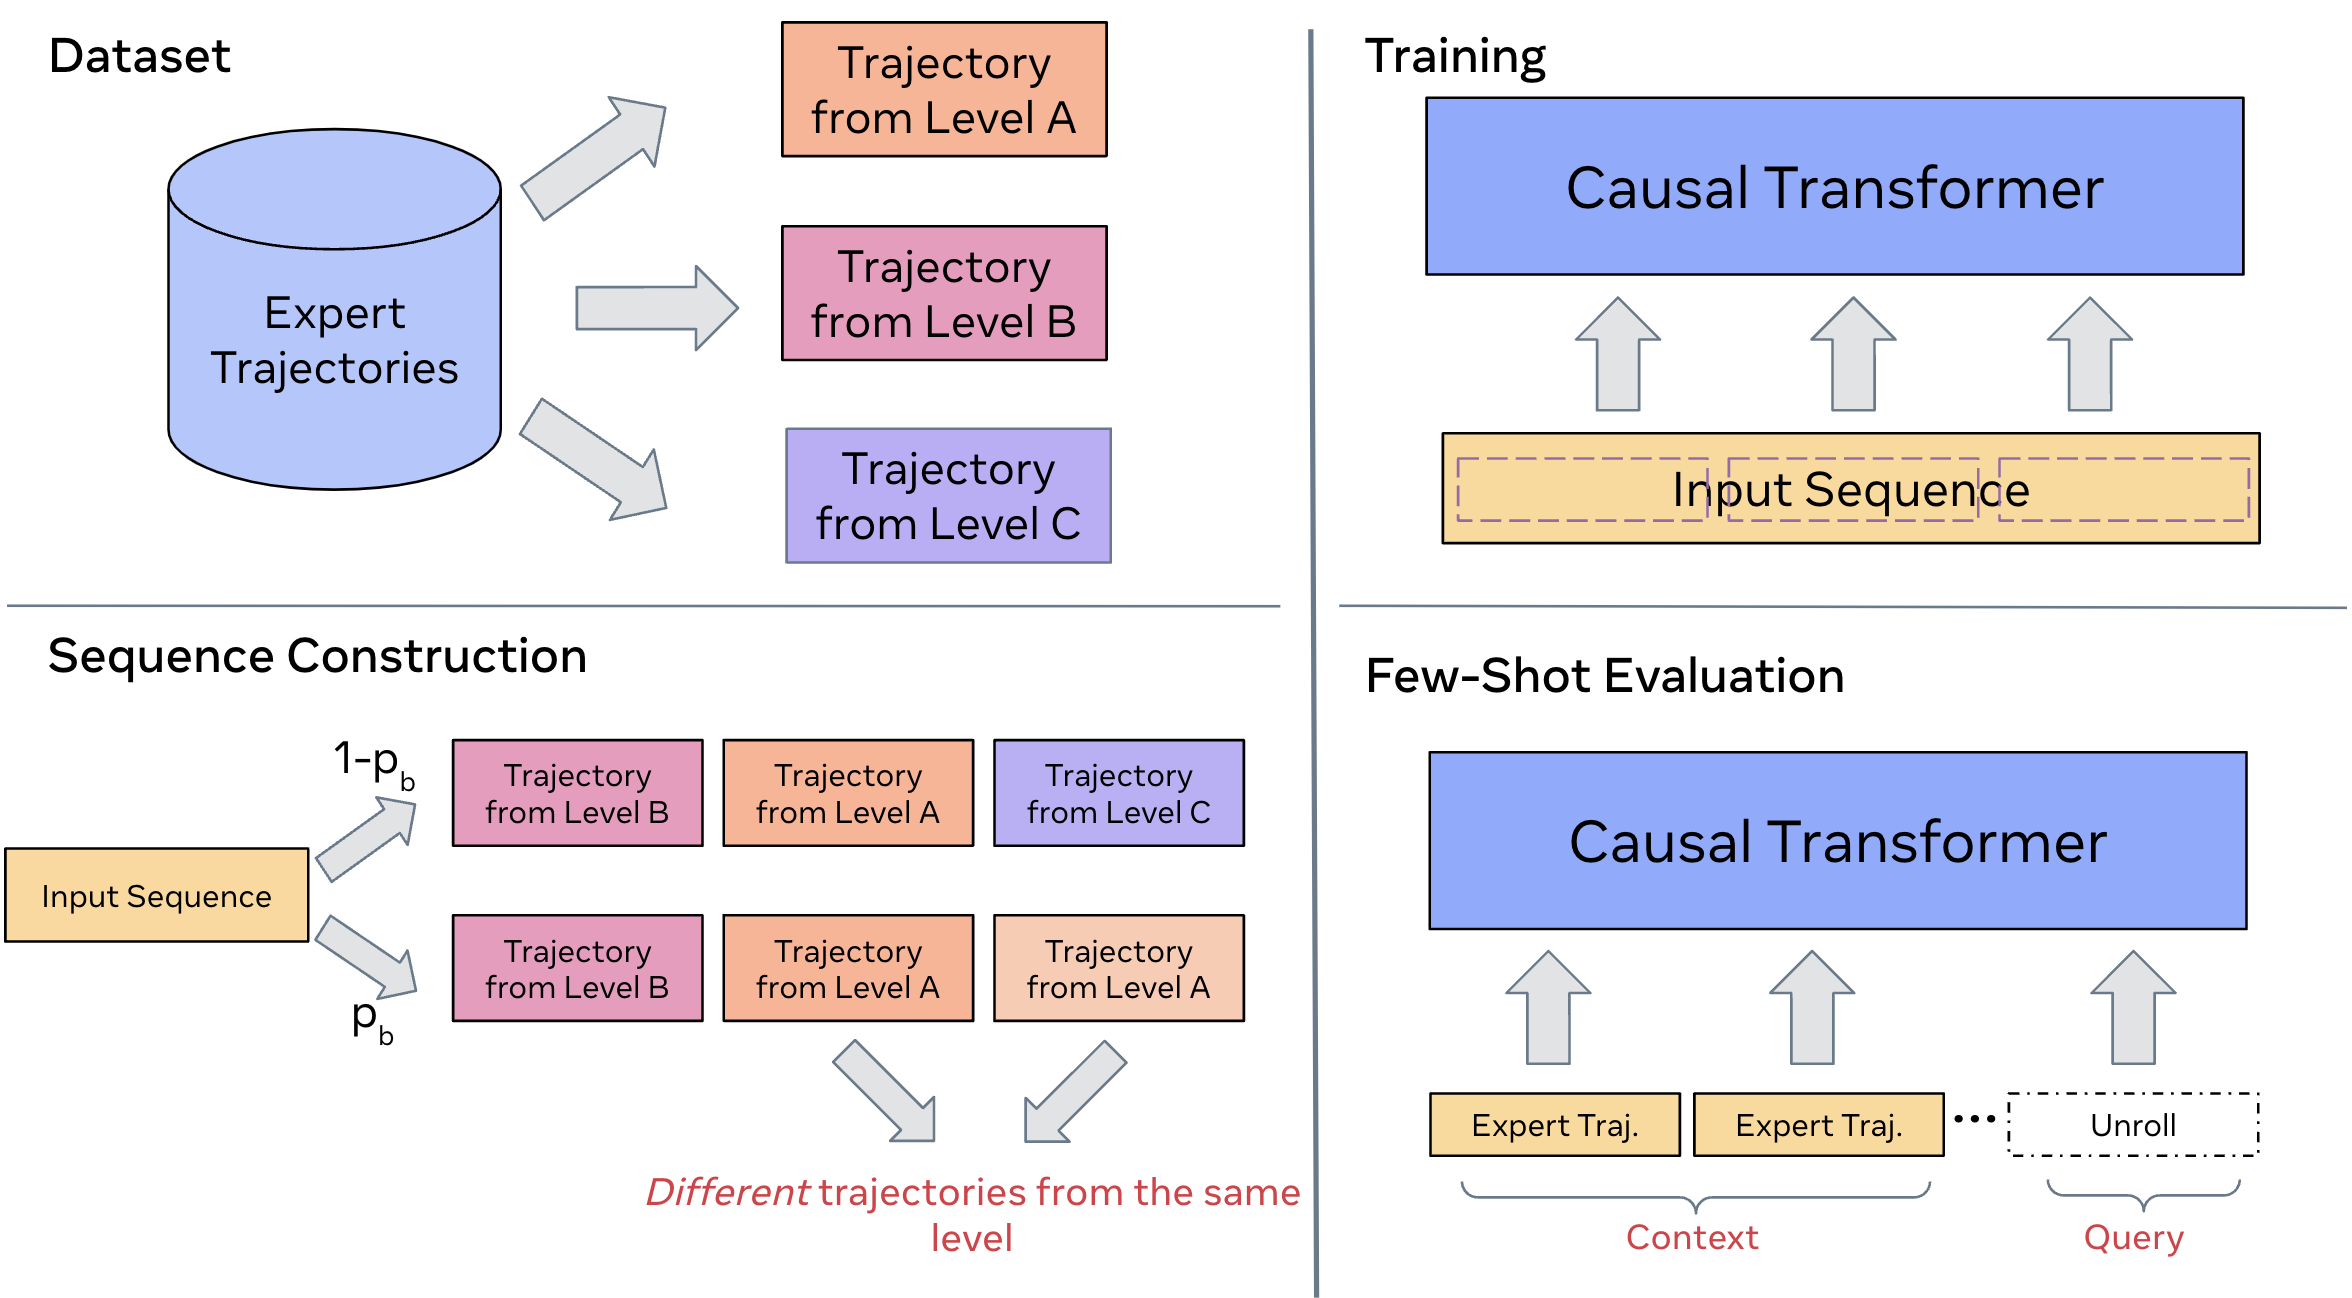
\includegraphics[width=\columnwidth]{figures/setup.png}
    \caption{\textbf{Experimental Setup:} We create a dataset of expert trajectories by rolling out expert policies
on $N$ tasks. Given these expert trajectories, we construct multi-trajectory sequences with
trajectory burstiness $p_b$. A sequence is bursty when there are at least two trajectories in the sequence from the same level. However, note that these trajectories are typically different due to the environment's stochasticity. These multi-trajectory sequences then serve as input to the causal transformer, which we train to predict actions. During evaluation, we condition the transformer on a few expert trajectories from an unseen task, then rollout the transformer policy until the episode terminates. }
    \label{fig:sequence_construction}
\end{figure}

\label{sec:methods}
\subsection{Training Data}
%\vspace{-2mm}
\label{sec:training_data}


\textbf{Tasks:} In order to study ICL for sequential decision making, we seek domains which are rich, diverse, and of varying complexity. For this reason, we decided to use MiniHack
\citep{samvelyan2021minihack} and Procgen \citep{cobbe2020leveraging}. MiniHack is a procedurally generated, dungeon-world sandbox based on the NetHack Learning Environment \citep{NLE} which provides a diverse suite of tasks exhibiting challenges related to navigation, tool use, generalization, exploration and planning.
Procgen, similarly to MiniHack, provides 16 procedurally generated game-like tasks to test the generalization abilities of the agent, and additionally features high-dimensional pixel-based observations. 
In MiniHack and Procgen, each ``level'' corresponds to a different random seed used to generate the task instance, including the layout, entities and visual aspects.

To generate our expert datasets, we used final checkpoints of E3B~\citep{E3B} policies for MiniHack and PPO~\citep{cobbe2020leveraging} policies for Procgen. Details can be found in  \ref{app:expert_data}. 


\textbf{Sequence Construction for Transformer Training: }
After collecting the expert data, we construct the trajectory sequences for training the transformer. Rather than using single-trajectory sequences as in the Decision Transformer model~\citep{decision_transformer} and its successors~\citep{traj_transformer, MGDT}, we use multi-trajectory sequences~\citep{adaptiveagentteam2023humantimescale, algo_dist}. We also remove the explicit conditioning on the episodic return and instead process the sequences in the form of $\{(s_0, a_0, s_1, a_1, r_1, \dots s_T, a_T)\}$ for each trajectory.


Moreoever, the multi-trajectory sequences adhere to certain distributional properties. First, we extend the concept of burstiness to the sequential decision making setting. Burstiness was first introduced in~\cite{zipfian_icl} to describe the quality of a dataset sample where the context contains examples that are similar to the query (for example, from the same class). Here, we extend this idea to \textbf{trajectory burstiness}, which we define as the probability of a given input sequence containing atleast two trajectories from the same level (\Cref{fig:sequence_construction}).This means that the relevant information required to solve the task is entirely in the sequence hence this design aids in-context learning. However, note that the trajectories, despite being from the same level, may vary because of the inherent environment stochasticity which means that the model still needs to generalize to handle these cases. These trajectories can be viewed as the sequential decision making equivalent of few-shot examples in supervised learning. To construct a bursty trajectory sequence, we sample $E$ trajectories from a given set of $L$ levels in such a way that, with bursty probability $p_b$, there are at least two trajectories coming from the same level. Note that all the trajectories within a sequence come from the same task. 


In our main experiments (\Cref{sec:main_expts}), we consider $p_b=1.0$, meaning that the context contains at least one trajectory from the same level as the query. Lastly, we shuffle the trajectories (and notably not the transitions within these trajectories) to construct a sequence of trajectories that will be used to train the transformer. \Cref{fig:sequence_construction} contains an illustration of our approach. 


\subsection{Model Training and Evaluation}
%\vspace{-2mm}
\label{sec:train_eval}
\textbf{Model Architecture and Training Procedure:}
For both MiniHack and Procgen, we use standard neural network architectures used in prior work~\citep{samvelyan2021minihack, cobbe2020leveraging} to process observations and use a separate embedding layer to process actions. 

In both cases, we then pass these sequences to a causal transformer ~\citep{vaswani2017attention}.  Finally, we use a cross-entropy loss over all the action predictions in our sequence. Unless otherwise specified, we use a 100M parameter transformer model for MiniHack and a 210M parameter model for Procgen.

\textbf{Evaluation:} We evaluate all the pretrained models on \textit{unseen} tasks that differ from those used during training, as shown in ~\Cref{fig:train_test}. For each pretrained model, we conduct two types of evaluations: few-shot and zero-shot. For few-shot evaluations, we condition the model on a handful of expert demonstration (ranging from 1 to 7) and roll out the transformer policy for five episodes. This is repeated for $L$ levels per task, and we aggregate the episodic return across all levels. The evaluation protocol for zero-shot evaluations is identical, with the exception that we do not condition on the expert demonstration. For all our results, we report mean and standard deviation across 3 seeds. 
